Una planta de tratamiento de agua necesita distribuir la máxima cantidad de agua desde un tanque de suministro (nodo \(so\)) hasta un tanque de recepción (nodo \(si\)). La red de tuberías conecta nueve nodos, y cada tubería tiene una capacidad máxima de flujo (en litros por minuto). Los nodos y las capacidades son los siguientes:

\begin{center}
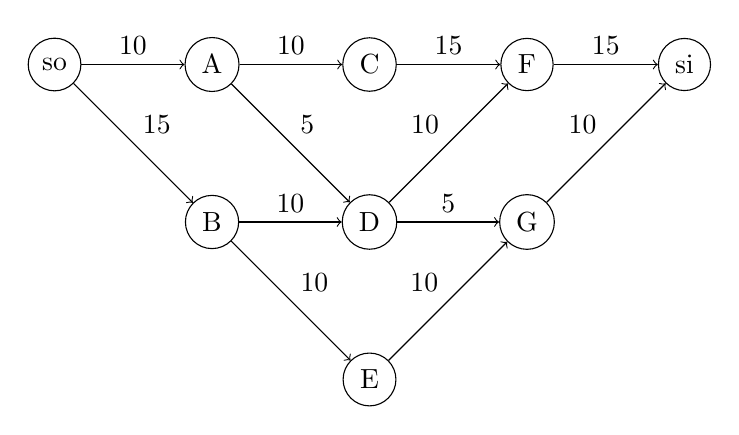
\begin{tikzpicture}[node distance=2cm, auto]
    % Nodes
    \node[draw, circle] (so) {so};
    \node[draw, circle, right of=so] (A) {A};
    \node[draw, circle, below of=A] (B) {B};
    \node[draw, circle, right of=A] (C) {C};
    \node[draw, circle, below of=C] (D) {D};
    \node[draw, circle, below of=D] (E) {E};
    \node[draw, circle, right of=C] (F) {F};
    \node[draw, circle, below of=F] (G) {G};
    \node[draw, circle, right of=F] (si) {si};
    
    % Edges with capacities
    \draw[->] (so) -- node {10} (A);
    \draw[->] (so) -- node {15} (B);
    \draw[->] (A) -- node {10} (C);
    \draw[->] (A) -- node {5} (D);
    \draw[->] (B) -- node {10} (D);
    \draw[->] (B) -- node {10} (E);
    \draw[->] (C) -- node {15} (F);
    \draw[->] (D) -- node {10} (F);
    \draw[->] (D) -- node {5} (G);
    \draw[->] (E) -- node {10} (G);
    \draw[->] (F) -- node {15} (si);
    \draw[->] (G) -- node {10} (si);
\end{tikzpicture}
\end{center}

Se pide:
\begin{enumerate}
    \item Determinar el flujo máximo de agua que puede ser transportado desde el nodo \(so\) hasta el nodo \(si\) mediante el método de Ford-Fulkerson.
    \item Identificar el corte con capacidad residual nula con los flujos obtenidos en el apartado anterior.
\end{enumerate}

